%\documentclass[journal]{vgtc}                % final (journal style)
\documentclass[review,journal]{vgtc}         % review (journal style)
%\documentclass[widereview]{vgtc}             % wide-spaced review
%\documentclass[preprint,journal]{vgtc}       % preprint (journal style)

%% Uncomment one of the lines above depending on where your paper is
%% in the conference process. ``review'' and ``widereview'' are for review
%% submission, ``preprint'' is for pre-publication, and the final version
%% doesn't use a specific qualifier.

%% Please use one of the ``review'' options in combination with the
%% assigned online id (see below) ONLY if your paper uses a double blind
%% review process. Some conferences, like IEEE Vis and InfoVis, have NOT
%% in the past.

%% Please note that the use of figures other than the optional teaser is not permitted on the first page
%% of the journal version.  Figures should begin on the second page and be
%% in CMYK or Grey scale format, otherwise, colour shifting may occur
%% during the printing process.  Papers submitted with figures other than the optional teaser on the
%% first page will be refused. Also, the teaser figure should only have the
%% width of the abstract as the template enforces it.

%% These few lines make a distinction between latex and pdflatex calls and they
%% bring in essential packages for graphics and font handling.
%% Note that due to the \DeclareGraphicsExtensions{} call it is no longer necessary
%% to provide the the path and extension of a graphics file:
%% 
\includegraphics{diamondrule} is completely sufficient.
%%
\ifpdf%                                % if we use pdflatex
  \pdfoutput=1\relax                   % create PDFs from pdfLaTeX
  \pdfcompresslevel=9                  % PDF Compression
  \pdfoptionpdfminorversion=7          % create PDF 1.7
  \ExecuteOptions{pdftex}
  \usepackage{graphicx}                % allow us to embed graphics files
  \DeclareGraphicsExtensions{.pdf,.png,.jpg,.jpeg} % for pdflatex we expect .pdf, .png, or .jpg files
\else%                                 % else we use pure latex
  \ExecuteOptions{dvips}
  \usepackage{graphicx}                % allow us to embed graphics files
  \DeclareGraphicsExtensions{.eps}     % for pure latex we expect eps files
\fi%

%% it is recomended to use ``\autoref{sec:bla}'' instead of ``Fig.~\ref{sec:bla}''
\graphicspath{{figures/}{pictures/}{images/}{./}} % where to search for the images

\usepackage{microtype}                 % use micro-typography (slightly more compact, better to read)
\PassOptionsToPackage{warn}{textcomp}  % to address font issues with \textrightarrow
\usepackage{textcomp}                  % use better special symbols
\usepackage{mathptmx}                  % use matching math font
\usepackage{times}                     % we use Times as the main font
\renewcommand*\ttdefault{txtt}         % a nicer typewriter font
\usepackage{cite}                      % needed to automatically sort the references
\usepackage{tabu}                      % only used for the table example
\usepackage{booktabs}                  % only used for the table example
%% We encourage the use of mathptmx for consistent usage of times font
%% throughout the proceedings. However, if you encounter conflicts
%% with other math-related packages, you may want to disable it.

%% In preprint mode you may define your own headline.
%\preprinttext{To appear in IEEE Transactions on Visualization and Computer Graphics.}

%% If you are submitting a paper to a conference for review with a double
%% blind reviewing process, please replace the value ``0'' below with your
%% OnlineID. Otherwise, you may safely leave it at ``0''.
\onlineid{1211}

%% declare the category of your paper, only shown in review mode
\vgtccategory{Research}
%% please declare the paper type of your paper to help reviewers, only shown in review mode
%% choices:
%% * algorithm/technique
%% * application/design study
%% * evaluation
%% * system
%% * theory/model
\vgtcpapertype{application/design study}

%% Paper title.
\title{Visualization of Technical and Tactical Characteristics in Fencing}

%% This is how authors are specified in the journal style

%% indicate IEEE Member or Student Member in form indicated below
\author{Mingdong Zhang, Li Chen, Xiaoru Yuan, Renpei Huang, Shuang Liu, and Junhai Yong}
\authorfooter{
	%% insert punctuation at end of each item
	\item
	Mingdong Zhang, Li Chen, Renpei Huang, Shuang Liu, and Junhai Yong is with Tsinghua University.
	\item
	Xiaoru Yuan is with Perking University.
}

%other entries to be set up for journal
\shortauthortitle{Zhang \MakeLowercase{\textit{et al.}}: Visualization of Technical and Tactical Characteristics in Fencing}
%\shortauthortitle{Firstauthor \MakeLowercase{\textit{et al.}}: Paper Title}

%% Abstract section.
\abstract{
	Fencing is a sport that relies heavily on the use of tactics. However, almost all existing fencing data analysis methods are based on statistical models, which are difficult to discover hidden patterns. Unlike the sequential game such as tennis and table tennis, fencing is a kind of simultaneous game, thus the existing sports visualization methods cannot work well on it either. In this work, we cooperate with experts in fencing to analyze technical and tactical characteristics in fencing competition. To meet their requirements, we design and implement an interactive visualization system for fencing competition data - FencingVis. The sequences of the fencers�� actions in the bout are first explored to find patterns of behaviors. Then a graph model is constructed to show the combination of the tactical behaviors. A tactical flow graph is further designed to show the graph model and multiple interactive ways are provided to explore it. We also provide a number of well-coordinated-views to supplement the tactical flow graph. They can display the information in the fencing competition from different perspectives and integrate organically with the tactical flow graph through consistent visual style and view coordination. We demonstrate the usability and effectiveness of the proposed system by two case studies. According to the expert feedback, our system can help analysts find not only the tactical patterns hidden in the fencing game, but also the technical and tactical characteristics of the contestant.%
} % end of abstract

%% Keywords that describe your work. Will show as 'Index Terms' in journal
%% please capitalize first letter and insert punctuation after last keyword
\keywords{Sports visualization, visual knowledge discovery, sports analytics}

%% ACM Computing Classification System (CCS). 
%% See <http://www.acm.org/class/1998/> for details.
%% The ``\CCScat'' command takes four arguments.

\CCScatlist{ % not used in journal version
 \CCScat{K.6.1}{Management of Computing and Information Systems}%
{Project and People Management}{Life Cycle};
 \CCScat{K.7.m}{The Computing Profession}{Miscellaneous}{Ethics}
}

%% Uncomment below to include a teaser figure.
\teaser{
	\centering
	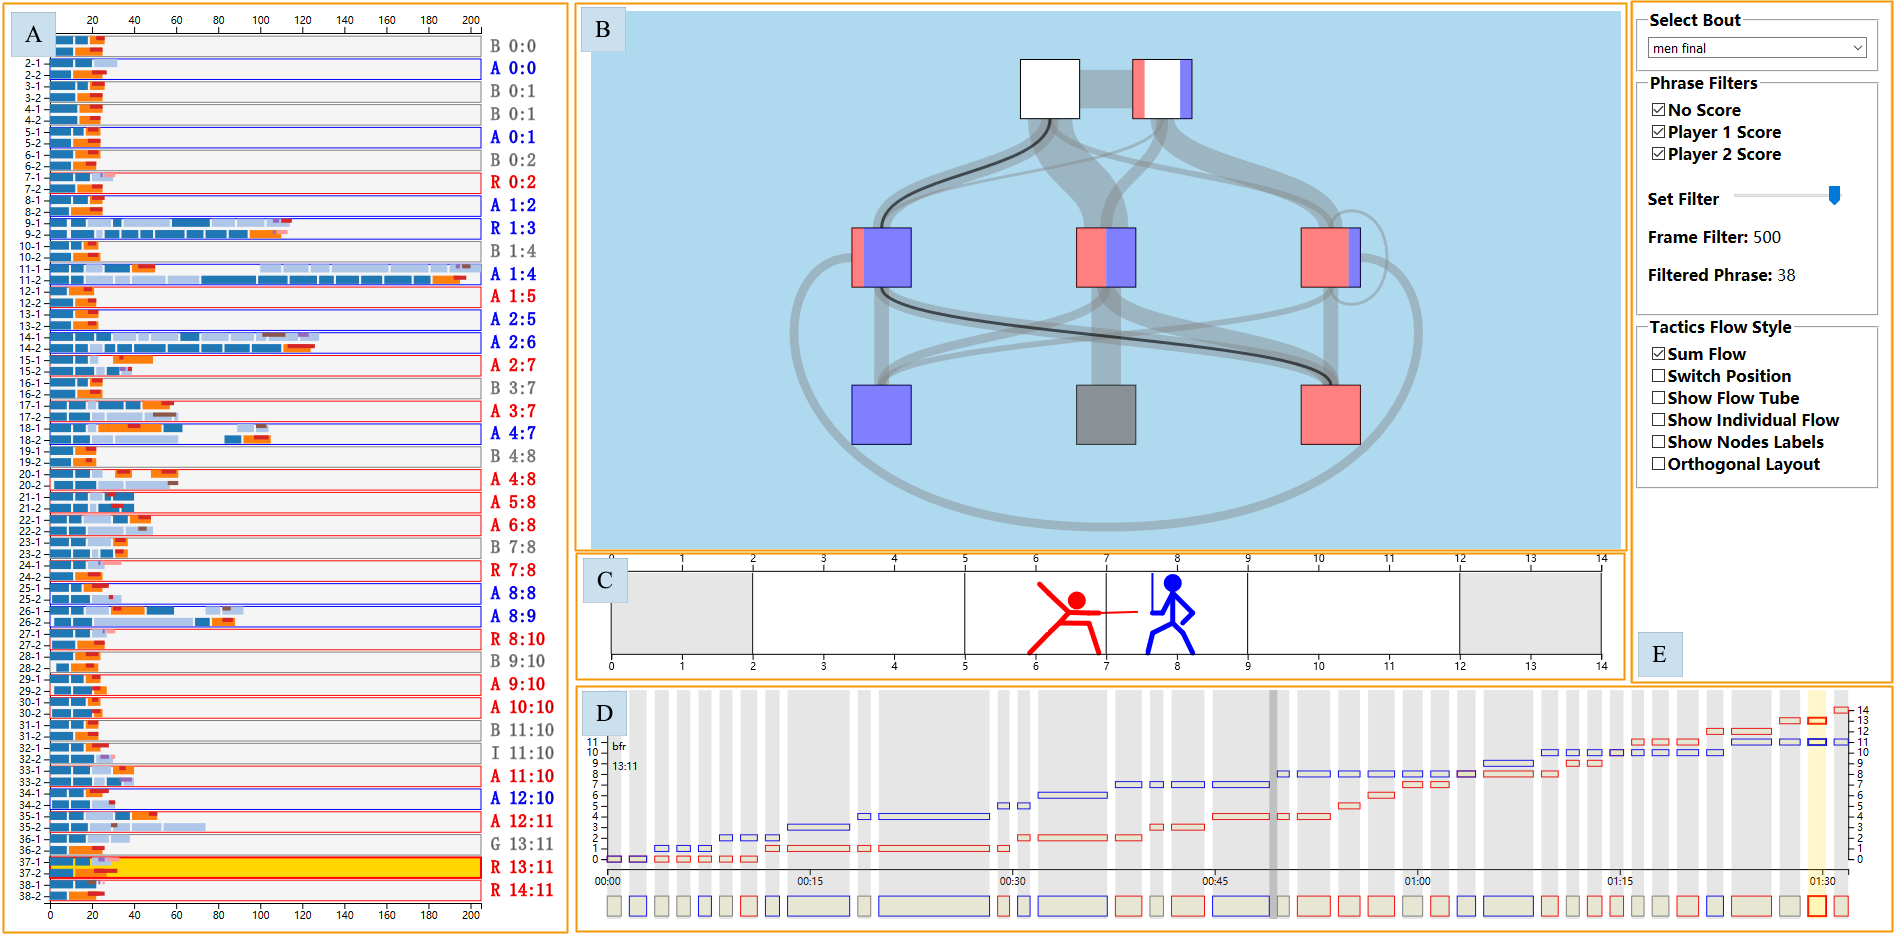
\includegraphics[width=\linewidth]{main}
	\caption{The main picture of FencingVis. A) Motion View. B) Tactic Flowchart View. C) Phrase View. D) Bout View. E Control Pannel}
	\label{fig:main}
}


%% Uncomment below to disable the manuscript note
%\renewcommand{\manuscriptnotetxt}{}

%% Copyright space is enabled by default as required by guidelines.
%% It is disabled by the 'review' option or via the following command:
% \nocopyrightspace

\vgtcinsertpkg

%%%%%%%%%%%%%%%%%%%%%%%%%%%%%%%%%%%%%%%%%%%%%%%%%%%%%%%%%%%%%%%%
%%%%%%%%%%%%%%%%%%%%%% START OF THE PAPER %%%%%%%%%%%%%%%%%%%%%%
%%%%%%%%%%%%%%%%%%%%%%%%%%%%%%%%%%%%%%%%%%%%%%%%%%%%%%%%%%%%%%%%%

\begin{document}

%% The ``\maketitle'' command must be the first command after the
%% ``\begin{document}'' command. It prepares and prints the title block.

%% the only exception to this rule is the \firstsection command
\firstsection{Introduction}

\maketitle

%% \section{Introduction} %for journal use above \firstsection{..} instead
Fencing has a long history and is one of the five activities which have been featured in every modern Olympic Games, however, participation in fencing has been relatively low.
This is due in part to the relatively high requirements for equipment and space and, more importantly, to the difficulty of learning.
It is difficult to learn mainly because it is not easy to understand.
Fencing is more abstract than other sports such as table tennis and tennis.
Let's take table tennis as an example. A table tennis match consists severl 7 games, each game is divided into multiple rounds, each round is divided into multiple strokes, and different strokes shows different stroke techniques.
But in a fencing bout, what happens in each phrase can't be clearly described.
In addition, fencing is a sport that relies heavily on the use of tactics. 
The adoption of reasonable strategies for different opponents can help the fencer increase the possibility of winning.
However, little research has been down on fencing data analysis, except for some based on some statistical models, which is not suitable for discovering tactics.
Therefore, visual methods are needed to help people better understand fencing competition, and find out the technical and tactical characteristics, so as to assist the training and the tactical arrangement of the competition.

There are many visualization methods for sports competition data before, but these methods can not be directly applied to fencing data.
Most of the sports data visualization methods are targeted at multiplayer sports, such as football and basketball, whose data show completely differect characteristics with data in fencing, and their methods can not be applied to fencing data.
For table tennis, tennis and other single-player sports, the characteristics of their back-to-back system lead to a clear hierarchy of data, which is not available in fencing data.
This determines that the visualization methods for them cannot be used for fencing data either.
As fencing competition data embodied in two related time series, we naturally think of some visual methods for time series comparison, such as that designed for bicycle sports\cite{beck2016matrix}.
However, the timing sequence of fencing data is not as simple as bicycle light movement.
The time series of fencing data contains the feature of tactics, and these features can not be extracted explicitly like in table tennis and tennis data, nor can they be extracted automatically from time series data like in bicycle data.
Due to this nature of fencing data, none of the above methods can be used directly for fencing data.

To fill this research gap, we cooperate with experts in fencing to analyze technical and tactical characteristics that are clear or fuzzy in fencing competition, and summarize the requirements of exploring these fuzzy problems through visual analysis. 
To meet these requirement, we design and implement an interactive visualization system for fencing competition data - FencingVis. 
We first analyze the sequences of the fencers�� actions in the bout. 
Then we extract the tactical behaviors and construct a graph model of these behaviors to express their tactical combinations. 
We design a tactical flow graph to show the model we built and provide multiple interactive ways to explore the tactical model. 
We also provide a number of well-coordinated-views to supplement the tactical flow chart. 
They can display the information in the fencing competition from different perspectives and integrate organically with the tactical flow graph through consistent visual style and view coordination.

We demonstrate the usability and effectiveness of the proposed system by two case studies. 
According to the expert feedback, our system can help analysts find not only the tactical patterns hidden in the fencing game, but also the technical and tactical characteristics of the contestant.
In addition to analyze professional competition, our system is able to use for the teaching to fencing beginners, and the tactical demonstration to fencing enthusiasts.


Our main contributions are as follows:
\begin{enumerate}
	\item We have structured definitions of fencing competition data and provide conversion from raw data to structured data.
	\item We design a variety of different views to present the transformed structured data in all directions and angles.
	\item We provide a series of interactive methods and view correlation to help professionals explore and find technical and tactical problems in the game, to better develop training plans and arrange the game strategy.
	\item We conducted user analysis of fencing athletes and coaches, as well as case studies of international competitions, which proved that our system could help them get new intuiation.
\end{enumerate}

\section{Related Work}
Our work is mainly related to the analysis of fencing data and sports data visualization and visual analysis, so we first introduce the related work in these two areas.

\subsection{Analysis and Visualization for Fencing}
The existing data analysis for fencing mainly focus on biomechanics category, through the analysis of competition data to send the difference between excellent fencers and beginners, so as to clear the focus of training\cite{chen2017biomechanics}. But these works are completely from the technical level, did not consider the improvement of tactical ability. 
Previous studies have also used statistical methods for time series analysis of fencing competition data\cite{tarrago2016complementary}. These studies use the existing empirical model to collect data, and the game process is summarized as a combination of several known patterns\cite{tarrago2015analisis}. We use this description of the game for reference, but at the recording level we choose to record the most primitive data, such as the movements of the steps and the movements of the hands. This can reduce the cost and information loss caused by introducing domain knowledge into the data acquisition process. We put the data abstraction work in the subsequent analysis process, doing so will bring a variety of benefits. First of all, the behavior pattern of different sword species is different, but at the most basic level is the hands and feet of all kinds of actions, we can use a unified format to record data, and in the logic of processing to distinguish it. In addition, if these empirical models change in the future, we can modify the logic of the system without having to recapture the data.

\subsection{Sports Visualization and visual analytics}
The visualization and visual analysis of sports data has developed vigorously in the past two decades, but there are still many opportunities and challenges.
Basole et. al. summarized two major difficulties in visualizing sports data\cite{basole2016sports}.
In addition to the complexity of the data, the main dilemma facing sports data visualization is the wide range of users, and different users' needs vary greatly.
Previous work has often targeted the needs of a particular class of users.
Some for general sports enthusiasts, some for professional athletes and coaches, some for related sports institutions and operators, some for psychological and physiological related researchers.

From the analysis of the data range, sports data visualization work can also be classified into four categories.
There is some work for a full tournament or league season, showing the points and rankings of each team during the season\cite{perin2016using}, or providing support for game forecasting\cite{vuillemot2016sports}.
The other is for a game, showing the dynamics of the situation in the game and the information on both sides of the game.
Some of the work is aimed at multi-player games, such as football, basketball, they focus on the spatial information of athletes, and analyze the space reflects the tactical layout of the impact on the game.\cite{sacha2014feature,perin2013soccerstories}.
Others focus on showing and analyzing the use of tactics or ability characteristics for individual athletes.\cite{polk2014tennivis,wu2018ittvis}
There are also games that compare multiple games. 
The last category deals with certain scenarios for a particular athlete or game.

Our work is for a single-player game, and two previous jobs are similar to our scenario.
TenniVis\cite{polk2014tennivis} uses the score and serve data to analyze amateur tennis matches.
iTTVis\cite{wu2018ittvis} uses more specialized data, such as placement and batting techniques, to analyze table tennis data more professionally.
Their method does not apply to fencing data because fencing has different characteristics compared to tennis and table tennis.
First of all, tennis and table tennis each round will end with one score, and fencing is not the case, some rounds can be both sides do not score, and some rounds both sides score (epee), which requires different visual design.
In addition, priority rules in fencing competition is very important, and the judgment of this information needs some professional knowledge.
If you can't judge the ownership of the priority, you can't understand the fencing score.
Therefore, the demonstration of priority is very important to the understanding of fencing competition.
We summarize the characteristics of fencing that need to be considered in visual design:
\begin{itemize}
	\item Fencing is not as easy to understand as tennis, table tennis, etc.
	It is often difficult for inexperienced users to read games directly.
	Therefore, the visual design needs to be able to help users better understand the game.
	\item In most sports competitions, the current field information is clear, but the most important priority information in fencing is not clear.
	People with different experiences may have different understandings, which involves the visualization of uncertainty.
	\item Most sports are bound to end each round with one side scoring, but fencing is not the case.
	Both sides may not score points or score points at the same time in a phrase, which also needs special design to reflect.
	\item The use of tactics is more important in fencing than in sports that place more emphasis on adaptability.
	And fencing tactics are often planned in advance before each phrase, so it is more valuable to show the impact of this strategy on the game.
\end{itemize}
In addition, fencing is divided into epee, foil, and sabre.
The three have both similarities and their own characteristics.
Therefore, showing the differences between the three is also one of the design goals of visualization system.


\section{Background and System Overview}
We will introduce the background knowledge of fencing, as long as the data we used and the analysis target. We will also give the main picture of our system.
\subsection{Background}
Fencing is one of the representative events of the Olympic games, which developed from the fencing used for military combat and duel in the cold weapon era.
Fencing consists of epee, foil, and sabre, all of which score by hitting the opponent's active part.
The basic techniques of fencing are divided into offensive techniques and defensive techniques.
Attack techniques include attack, riposte, feint, lunge, beat attack, disengage, compound attack, continuation/renewal of attack, and flick.
Defense techniques include parry, circle parry, counter attack, point-in-line.
These techniques are implemented by a limited combination of hand and foot movements.
Fencing competition is divided into individual and group competition, there are two stages of group competition and group competition.
The individual's first 15 points out of the group game to win ( heavy sword or foil after playing full game time score more victory ).
After one player has scored eight points in the sabre match, the two sides will take a minute off.



\subsection{Data Description}
Because of the fast pace of fencing, it is difficult to record the details of the match in real time.
And in order to avoid interfering with the competitors, it is not convenient to install the sensor device.
The existing analysis of fencing competition is achieved through the video of the game, we also extract data from the game video data.
Because of the accuracy of the general game video is 30 frames per second, we record data frame by frame, time accuracy is 1/30 seconds. For each frame of data, we record the listing attributes:

\begin{table}[]
	\centering
	\caption{Data Description}
	\label{my-label}
	\begin{tabular}{|p{2cm}|p{4cm}|}
		\cline{1-2}
		Bout ID  &  The ID of the bout to which this event belongs.\\	\cline{1-2}
		Phrase ID  & The ID of the phrase to which this event belongs.\\	\cline{1-2}
		Frame  &  The frame at which this event occurs.\\	\cline{1-2}
		Footwork of Fencer 1  & Begining or finishing of forward, backward, or lunge of fencer 1\\ 	\cline{1-2}
		Footwork of Fencer 2  & Begining or finishing of forward, backward, or lunge of fencer 2\\ 	\cline{1-2}
		Bladework of Fencer 1  & Begining or finishing of attack, parry, piposte, or counter attack of fencer 1\\ 	\cline{1-2}
		Bladework of Fencer 2  & Begining or finishing of attack, parry, piposte, or counter attack of fencer 2\\ 	\cline{1-2}
		Attack Position of Fencer 1  & Attacked position of fencer 1\\ 	\cline{1-2}
		Attack Position of Fencer 2  & Attacked position of fencer 2\\ 	\cline{1-2}
		Parry Position of Fencer 1  & Parried position of fencer 1\\ 	\cline{1-2}
		Parry Position of Fencer 2  & Parried position of fencer 2\\ 	\cline{1-2}
		Confrontation position  & Confrontation position of the two fencers on the strip.\\ 	\cline{1-2}
		Result  & The referee's decision on the current phrase.\\ 	\cline{1-2}
		Score  & Record which player scored or none.\\ 	\cline{1-2}
	\end{tabular}
\end{table}

In the process of data marking, continuous footwork is not easy to effectively segmentation.
After consulting the domain experts, we use the start time of the next action as the segmentation point of the two actions.
Such as continuous forward we use each front foot lift as a segmentation point, continuous back we use each rear foot lift as a segmentation point.

\subsection{Requirement Analysis}
Through ongoing exchanges and discussions with field experts, we have initially identified system needs:
\begin{itemize}
	\item (R1) Show how the game changes over time
	\begin{itemize}
		\item (R1a) Show changes in scores
		\item (R1b) Shows how long each turn lasts
	\end{itemize}
	\item (R2) Show a detailed comparison of the actions of each phrase
	\item (R3) Show how the tactics of both sides were used throughout the game
	\item (R4) Exploratory pattern discovery and result communication
\end{itemize}
\subsection{System Overview}
Our system consists of five forms, as shown in \autoref{fig:teaser}
\section{FencingVis}
\subsection{Bout View}
Almost all game data naturally have time attributes, and both tactical and technical analysis need to consider the impact of time.
The influence of time is reflected in two aspects.
First of all, different stages of the game, the athlete's psychological and physical changes, which has an important impact on the results of the game.
In addition, the use of tactics is also time - dependent.
The fencer will choose the next tactics based on the tactics he or she and his or her opponent have used over a period of time.
Such as the choice of repetition or conversion, need to be determined according to the characteristics of the previous game and the opponent.
Therefore, it is very important for analysts to show the changes of competition over time.

The bout view mainly shows three elements, time, score change and phrase duration.
We use a tailored step chart to show the variation of scores according to time.
X - axis mapping game time, y - axis mapping score.
Red and blue rectangles represent scores for both sides, respectively.
The two rectangles naturally overlap in purple when they are equal-scored.
To visually compare the duration of each turn, we add a horizontal rectangle below the x - axis to show each phrase.
The color of the rectangle indicates the player who scores in this phrase, and the gray indicates that neither side scores.
The upper and lower views correspond to each other, helping the user visually observe the relationship between the three attributes.
Since the break between the first and second half often has a greater impact on the course of the game, we use a vertical line to emphasize this split moment.
When making a selection of the phrase, we use a gray background to reflect the selection of the phrase.

Description: The game time in our view does not exactly correspond to the natural time.
Since the time in the fencing phrases accounts for a small proportion of the actual time, the view becomes very sparse if mapped directly.
So we map the time in the phrases equally, and map the time between two adjacent rounds all to one second interval.

\subsection{Motion View}

\begin{figure*}[tb]
	\centering
	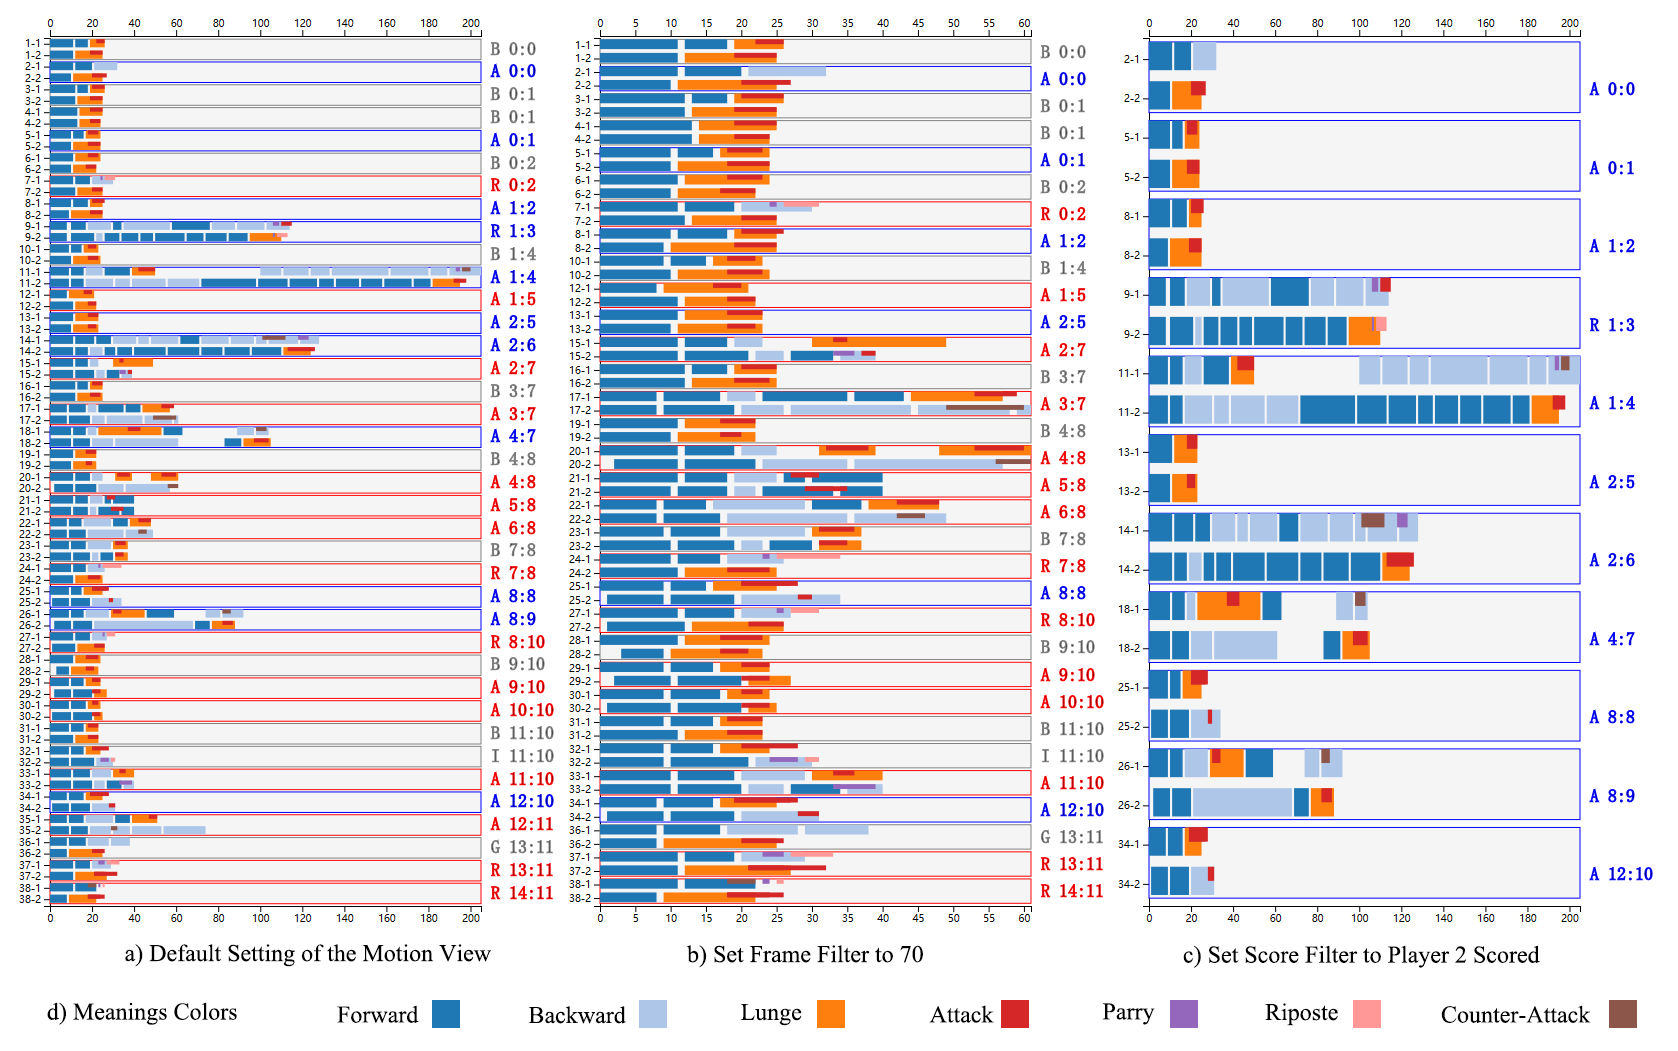
\includegraphics[width=\linewidth]{motionview}
	\caption{Motion View}
	\label{fig:motionview}
\end{figure*}

The motion view is mainly used to show the details of the clash between the two swordsmen in each phrase.
Phrases are arranged row by row from top to bottom in the order of the game, with each row describing the information for one phrase.
Each phrase is subdivided into two lines up and down, respectively, describing the action of two fencers, with the left fencer in the above, and the right fencer in the below.
Labels to the left of each phrase boxe indicate the order of the current phrase and the corresponding fencer for quick retrieval.
And the labels on the right show the outcome of each phrase. We use the first letter to show the  words of the referee(A for attack, R for riposte, S for simultaneous), along with the outcome scores.

Bar charts are used to describe fencers' behaviors within the turn, the horizontal axis corresponds to time duration, which is described by the number of frames.
We use data from videos containing 30 frames per second, so the scale is the same.
If the corresponding number of seconds is needed, it can be viewedfrom the corresponding location  in the bout view.
Tall bars indicate the movements of the feet, and short bars embedded in the tall bars indicate the swordwoks. Different colors stand for different type of actions, which is shown in c of \autoref{fig:motionview}.

In order to highlight the score of the phrase, we use the colorsof the two fencers (red and blue) to render the border and text of the phrase respectively.
The non - coloring of the fill is done to avoid interfering with the display of internal details, which, if translucent, can lead to color inconsistencies.

The items shown in the motion view is affected by the filter setting in the control panel, which including score filters and duration filters.

\subsection{Tactic Flow View}
\begin{figure*}[tb]
	\centering
	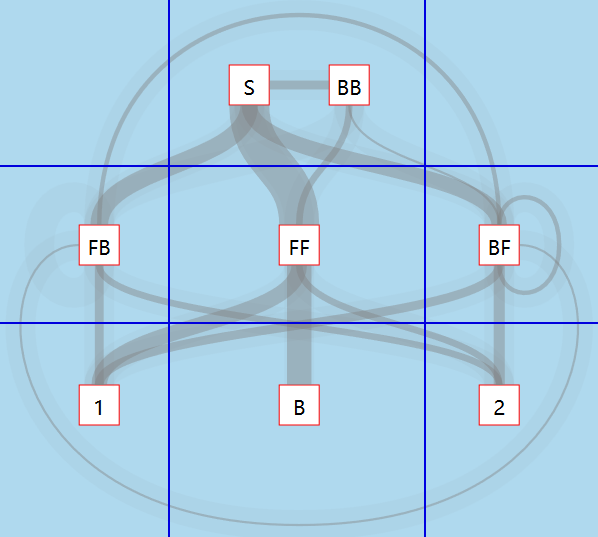
\includegraphics[width=\linewidth]{flowchart}
	\caption{Tactics Flow View}
	\label{fig:flowchart}
\end{figure*}
Only time series and statistical level display, can only let the user more clear understanding of the game, does not bring more inspiration.
In order to allow analysts to have a deeper understanding of the tactical use of both sides in the game, we designed a tactical flow chart to show the tactical use of two fencers.

In order to analyze the tactical information in fencing competition, we first convert the collected time series torque into a tactical graph model.
We consulted professional fencing coaches and athletes and devised a series of conversion rules.
The process of modeling needs to introduce some domain knowledge, not directly from the level of data conversion.
For example, to check whether the fencer choosing forward orbackward strategies, we need to look at the behavior after the first two or more steps.
The use of strategy itself is a process of deception and anti-deception\cite{roi2008science}. Fencer usually use two-step lunge, but sometimes will also use one-step lunge in order to attack in sudden. So there may be one-step lunge, but most backword movements are performed after two steps forward.

The design of tactical flow chart is based on the graph model we built for the game data.
Through in-depth discussion with experts, we abstract the time series of fencing competition into eight States:
\begin{enumerate}
	\item Start(S): This is the state when the referee issues a start command, with both sides behind the engard lines (or the position where the last phrase interrupted). 
	The start state is the first state of the dataflow graph for each phrase and the source node of the dataflow graph.
	\item Forward-Forward(FF): This is the state of both sides to attack forward at the same time.
	The game enter this state in two scenarios. 
	After the start of both sides attack into ff state at the same time or both sides back at the same time and then switch into ff state at the same time.
	\item Backward-Backward(BB): This is the state of simultaneous retreat.
	Since both fencers will step forward after the start in most case of the fencing phrase, our decision on BB state is not according to a direct backwards, but whether a backward is planned before the phrase. 
	It is usually the case that both fencers perform a step or two forward, then switch to back away.
	If the fencer pauses as he moves forward and then moves on, we also determine that he chooses backward tachtic, though with a fast switching.
	\item Backward-Forward(BF): The state that the left fencer chooses backward while the right fencer chooses forward.
	\item Forward-Backward(FB): The state that the left fencer choose forward while the right fencer choose backward.
	\item Player 1 score(1): The state that fencer 1 score.
	\item Player 2 score(2): The state that fencer 2 score
	\item Simultaneous(S): The state that both fencers hit each other simultaneously without any scoring.
\end{enumerate}

In order to provide a more intuitive observation, we arranged the nine nodes according to the following criteria:
\begin{itemize}
	\item The view shows the progress of the game from top to bottom.
	The nodes are naturally arranged in three layers.
	The first layer, containing node S and node BB, is designed to represent the start of the phrases.
	The second layer, containing node FB, node FF and node BF, is used to represent the middle stage of the phrases.
	The third layer which contains node 1, node 0, and node 2, is to represent the end of the phrases.
	All data flow in that data flow diagram flow only from the upper layer to the low layer or between the same layers.
	\item The node layout of the view in the horizontal direction reflects the advantages of the fencers.
	The nodes are arranged in three columns.
	The left column indicates that the player on the left are dominant (scoring or having priority).
	The right column indicates that the player on the right are dominant.
	The middle column represents the balance of power between the two sides.
	\item Although we've laid out this principle as a whole, we've made some trade-offs to keep our views clean and tidy.
	Such as node S and node BB, which should be arranged up and down if strictly in accordance with the above rules, are arranged in the same horizontal layer. 
	Otherwise, there will be a lot of overlap.
	We arrange the two nodes left and right, but close together as one region, this is is consistent with the above rules in the region level.
	This can also make the edge between the node S and node BB in a focused position (center on the upper side), which can show the importance of this edge (as discussed in the case studies).
	
\end{itemize}
In order to compare the two fencers' tactical behaviors, we also designed two simplified flow charts for each of the two fencer's tactics, as shown in a) and c) of \autoref{fig:flowchart}

\subsection{Animation Replay}
\begin{figure*}[tb]
	\centering
	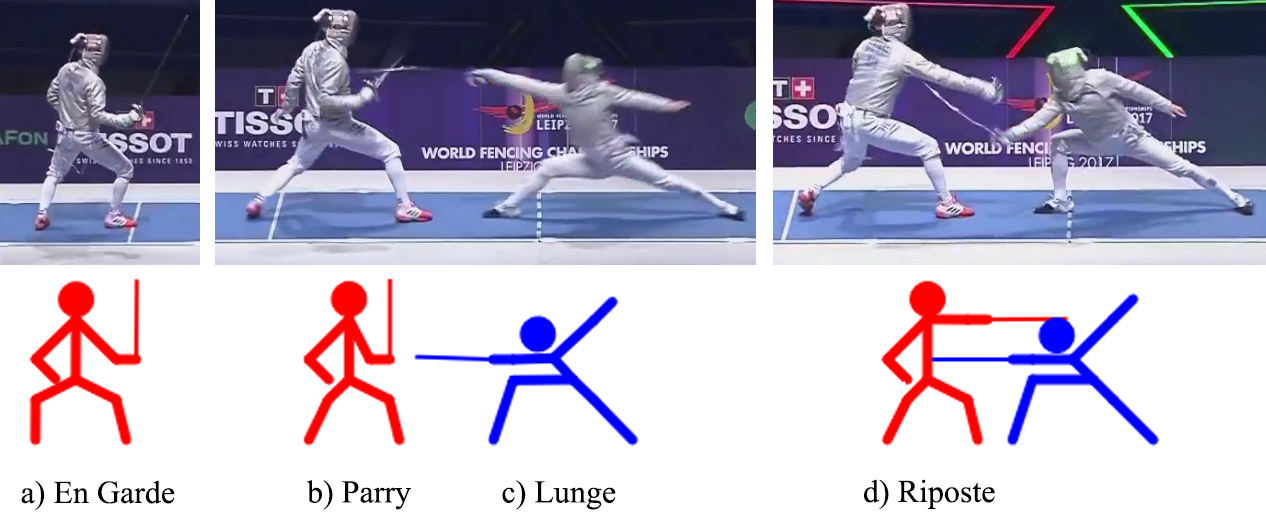
\includegraphics[width=\linewidth]{glyph}
	\caption{Glyph designing of the animations in the phrase view}
	\label{fig:sample}
\end{figure*}
Although the phrase view shows the details of each phrase, its presentation is time-dimensional, which has two limitations.
The first is the inability to reflect the position information on the pitch, and this is not intuitive for domain experts.
To make up for this deficiency, we designed a phrase view to show the information of each round in the form of animations.

Our animation design mainly reflects two aspects of information, which are the position on the field and the attitude of both sides.
These two aspects of the information, although relevant, can be disassembled.
We use a more flexible design, animation design for two layers, respectively, to achieve the change of two kinds of information, stacked together to show the information of a phrase.
The animation of the position is relatively simple to implement, i.e. the position of the icon is driven against the recorded position data.
For pose animation, we abstract the player's pose on the pitch into four icons by observing existing games and consulting domain experts.
\begin{itemize}
	\item engarde glyph
	\item lunge glyph
	\item parry glyph
	\item riposte glyph
\end{itemize}
Animation is triggered by clicking on the corresponding turn in the behavior view,  which establishes a seamless connection between the two views.

\subsection{Control Pannel}
In order to meet the interactive exploration of data, we provide some control components, mainly used to filter and change the display mode of the displayed data, as shown in E of \autoref{fig:main}.
First of all, we provide a drop-down menu to select the game to analyze.
We also provides filters for the phrases, mainly from the results and time dimensions.
The result filters are used to select combinations that showing scoring phrase of player 1, scoring phrase of player 2 or no score phrases.
The time filter selects a time threshold through a time bar, and phrases with durationturns longer than the threshold are filtered out, leaving only short phrases.
The effects of the two filters can be superimposed and the results are updated synchronously on the bout view and the action view.
In order to have a clear understanding of the number of filtering results at all times, the filtering threshold and the number of filtered results are displayed simultaneously.

Controls of the display mode provides selection of three modes.
The user may choose whether the data stream displays the entire game or makes a comparison between the first and second halves.
Users can also choose to exchange the position of the fencers, which is used in the scenario that  different games of the same player need comparison. If a fencer is located on different sides in these gamey, data flow chart comparison is not intuitive for comparison, and switch to the same direction can make it easier.
The background of the data stream can also be chosen to be presented or not.
For users who have just come into contact with the system, the background presentation allows them to know more quickly which nodes can have data flow between them, although the current race under analysis may not have occurred.



\subsection{Interaction}
\subsection{Cross-View Analysis}
The interactive exploration of data is mainly realized through the association of views.
The main view associations we provide are the following:
\begin{itemize}
	\item After the user modifies the filter settings, the action view and game view are updated synchronously.
	The former displays only the filtered results, while the latter highlights the filtered results with a gray background.
	\item When the mouse moves in the action view or the bout view, the corresponding phrase of the two views highlights the border to prompt.
	The data flow for this round is also displayed synchronously in the data flow diagram
	\item User can click the items in action view or bout view to trigger the animation in the phrase view of the corresponding phrase.
\end{itemize}
\section{Case Study}
\subsection{Men's Sabre Individual Golden Match of 2017 World Fencing Championships}
In the first case, we will analyze the final of szatmari and gu in the men's individual men's fencing competition at the 2017 world championships.
Through a quick look at the bout view, we saw Gu leading in the first half, but Szatmari reversed in the second half, so we judged that the game's win and loss was related to a change in strategy in the first half and the second half.
So we switched the tactical flow chart to the half-court view, as shown in a) of \author{fig:case1}
\begin{figure*}[tb]
	\centering
	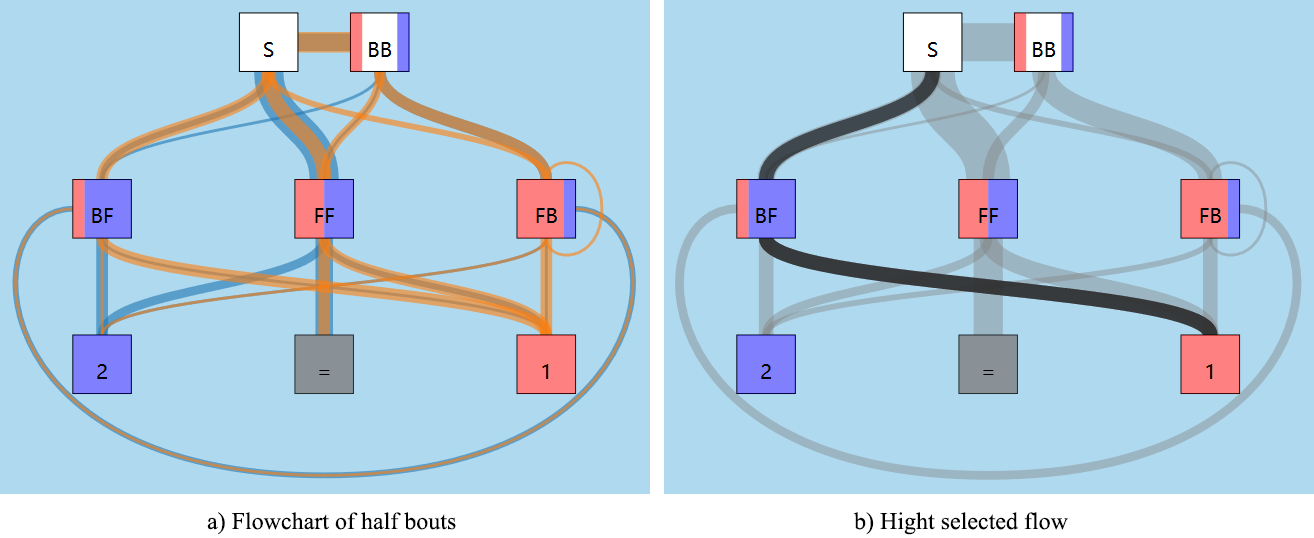
\includegraphics[width=\linewidth]{case1}
	\caption{Tactics flowchart of the first case.}
	\label{fig:case1}
\end{figure*}

We can see clearly that most of Gu's score in the first half came from FF and BF (shown in blue), which, however, was significantly reduced in the second half (shown in red).
At the same time, Szatmari's second-half main scoring sources were FB and BF nodes.
Summing up the four more obvious flow changes, we get the following preliminary conclusions:
\begin{enumerate}
	\item Gu's counter-attack points were reduced in the second half.
	\item Szatmari increased his score by moving forward while the his opponent choosing backward in the second half.
	\item Gu's forward with Szatmari's backward mainly contribute to Gu's score in the first half , but changed to contributing Szatmari in the second half.
\end{enumerate}
For these three preliminary conclusions, we try to find a deeper reason.
We shifted our attention from the lower half of the tactical flow chart to the upper half.
First, it is very intuitive to see that the S-FB flow increased in the second half and the S-FF decreased in the second half, both of which reflected Szatmari's progress, but Gu was backward and forward, respectively.
This means that Gu's progress in the second half decreased, back increased, which led to his points.

In addition, we observed the inflow of BF node, S-BF increased in the second half.
In order to further analyze the situation of BF node, we switch back to the overall tactical flow chart to select the S-BF segment, as shown in b) of \autoref{fig:case1}.
At this point we can see that most of the S-BF flow ended up at node 1, which is Szatmari scoring, and most of these were occurred in the second half.

So we can get a guess at the game:
\begin{enumerate}
	\item Gu led the game with points in the first half, relying on his strong offensive ability.
	Szatmari failed to handle Gu's attack, 	no matter choosing forward or backward.
	\item After the break, Szatmari adapted to Gu's attack, and began to retreat to catch Gu's attack, and achieved success, scored many times, which is reflected in the BF-1 segment.
	\item As a result of being caught many times,Gu's attack began to hesitate, chose more backward.
	This is reflected in the decrease in counter-attack and the increase in Szatmari's forward Gu retreat.
	\item Together, these factors led to gu's defeat.
\end{enumerate}
In order to confirm the above assumptions, we locate the start phrase of the second half in the game view, and then check the details of the next few phrases in the motion view.
From the action view, we see that Szatmari consecutive offensive points in the phrases of beginning of the second half, which is different with our previous assumptions.
At the same time, Szatmari's backward scorings came at the end of the game.
So we redefined our understanding of the game:
\begin{enumerate}
	\item Gu led the game with points in the first half, relying on his strong offensive ability.
	\item However, although Gu attack sharp, but its attack on the physical consumption is bigger, after the start of the second half, its attack effect began to weaken, leading to the opponent's attack score.
	\item So Gu began to change strategy, the use of retreat began to increase, however, its ability to retreat is not good at, so was chased points by his opponent.
	\item Gu had to continue to attack, but because the opponent has seen its speed decline, continuous retreat to catch its attack, and finally won.
\end{enumerate}

We analyzed gu's tactics and tactics through this game.
His offensive ability is very strong, but the attack on the physical loss is too big, lead to the second half is unsustainable.
If gu wants to improve, he needs to strengthen his strength to keep the offensive ability does not decline, or improve his other aspects of the short board, also can have other effective method in the case of attack ability decline.
From szatmari's point of view, its ability is relatively average, the second half of the timely discovery of the opponent's state changes, reasonable adjustment strategy, and achieved the final victory.


\begin{figure*}[tb]
	\centering
	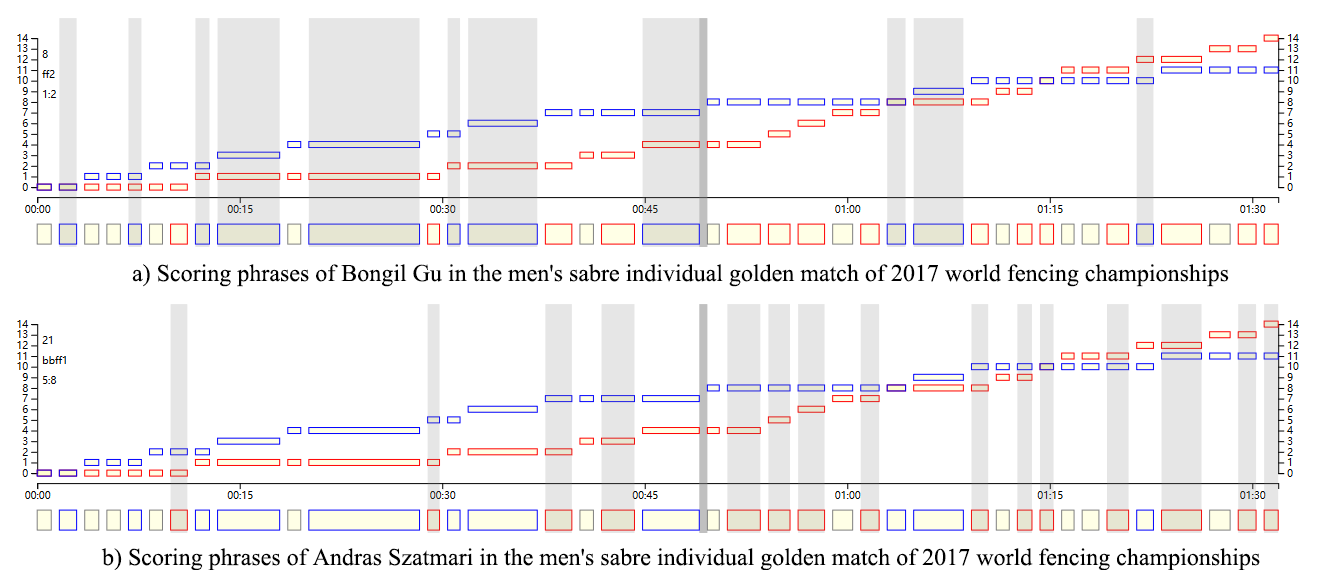
\includegraphics[width=\linewidth]{ScorePhrases}
	\caption{Bout View}
	\label{fig:boutview}
\end{figure*}
Finally, let's check the scoring rounds phrases of both fencers in the game view respectively.
It is clearly shown in \autoref{fig:boutview},  all long duration phrases contributed to Gu's scoring (shown in a)), while szatmari's scoring phrase are all short phrases (shown in b)).
This also confirmed that Gu's ability is better, Szatmari won the game  through reasonable tactical use.


\subsection{Comparison of Three Bouts}
\begin{figure*}[tb]
	\centering
	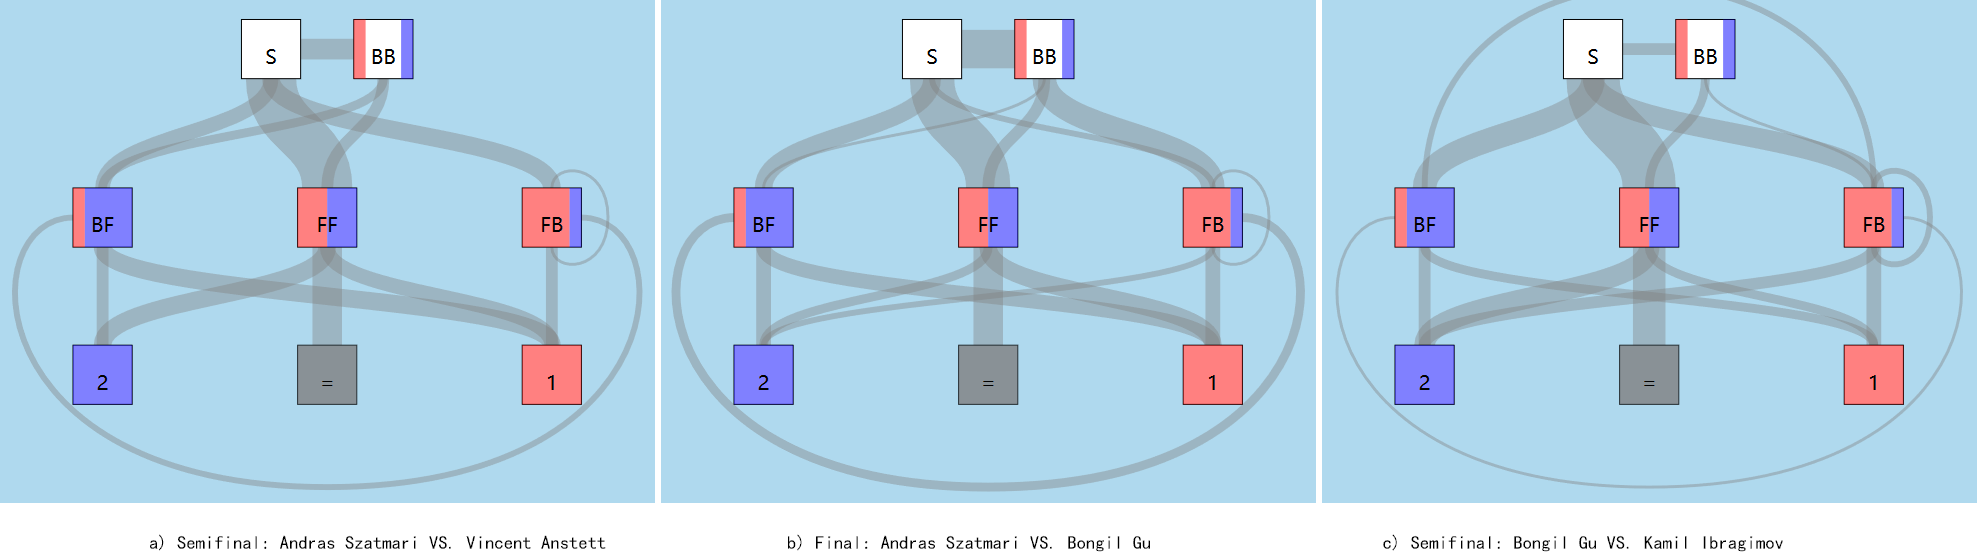
\includegraphics[width=\linewidth]{threeBout}
	\caption{Comparison of tactical flow charts in the semi-finals and finals of fencing world championships in 2017}
	\label{fig:sample}
\end{figure*}
In this case, we compared the tactical flow charts of the two semi-finals and final of the men's sabre individual at the 2017 fencing world championships.
For ease of comparison, we switched the position of gu and iburagimov in the semi-final, so the two fencers Szatmari and Gu we focused on were in the same position on the graph in their respective two games.

In the view, the thickest flow always catches the viewer's attention first.
Obviously, the flow S-FF is the thickest in all the three graphs, which is consistent with the dominant position of the attack in the sabre.
In addition, the flow S-BB in the final was significantly thicker than the corresponding flow in the two semi-finals, indicating that the fencers played more conservatively and  chose to retreat more frequently in the final.

Comparing the three games, szatmari's victory in the final mainly depends on the counter-attack score and back direct score, while in the semi-final mainly depends on the counter-attack score.
In the other semi-final, Gu's main way to score against his opponent was by going back and scoring directly.
It can be found that the main winning means in the sword game is to attack and pull open direct attack, and the formation of long-distance attack is less and rarely reflects the obvious advantages.
This show especially in high level competition, when the fencers' basic skills are equal.

This case showed shat our system can easily compare different games, which was not available in previous work\cite{wu2018ittvis,polk2014tennivis}



\section{Discussion}
During the design and development of the whole system, we refer to the development process model proposed by Sedlmar et al.\cite{sedlmair2012design}
But we still encountered a lot of problems.
At first we saw that the fencing data were two related time series data, so we initially planned to use the time series data analysis method directly, which is the approach widely accepted by other previous analyses of fencing data.
However, with the further understanding of the problem, we found that the time series data of fencing has a potential hierarchical structure.
The same motion series in different stages of the phrase reflect different technical and tactical information.
For example, two fencers always choose to move forward at the beginning of the phrase, and there are only one or two steps forwrd in this stage according to our statistics.
One or two steps in the initial stage of the phrase are closely related to the technical characteristics and tactics chosen by the fencers, and will have a great influence on the following competitions.
In contrast, after entering the long-distance attack and defense, the number of forward and backward steps is often not important, but the timing and depth of the lunge will have more important influence.

So we analyze the data from two levels.
We first represent the time series data of a phrase as a sequence of tactical combination behaviors from a higher level of abstraction, which reflects the tactical application of both fencers in this phrase.
Then in each node of the sequence, we analyze the technical ability of both sides, such as reaction time, attack position, etc.
Previous studies often analyze the technical capabilities of the entire sequence directly, however, according to our research, more detailed patterns and features in the data can be found by analyzing in this multi-layer framework.
Based on this hierarchical structure, our data presentation and interaction is also designed as two abstract levels to show tactical information and technical information respectively .
But our focus is still on the tactical level. 
There has been a lot of work focus on analyzing the technical characteristics, and we hope to be able to give analysts a new perspective under the tactical framework to understand the technical characteristics of the fencers.


\section{Conclusion}
We design and implement a visual analysis system fencingVis, for fencing data.
We use multiple views to present fencing data from different perspectives and provide exploratory analysis to domain experts through a series of interactive filters and view associations.
Through two case studies, we prove that the system can help domain experts find the patterns that are not easy to find before.
Experts also gave us a lot of positive feedback.

This system is mainly aimed at sabre individual.
The rules for epee and foil are slightly different, so we're going to improve the system for the other two types of sword.
At the same time, also want to add team game analysis.
Team events involve more players and the order between them adds new complexity to the data, which is also a problem we need to work on in the future.




%% if specified like this the section will be committed in review mode
\acknowledgments{
The authors wish to thank A, B, and C. This work was supported in part by
a grant from XYZ (\# 12345-67890).}



%\bibliographystyle{abbrv}
\bibliographystyle{abbrv-doi}
%\bibliographystyle{abbrv-doi-narrow}
%\bibliographystyle{abbrv-doi-hyperref}
%\bibliographystyle{abbrv-doi-hyperref-narrow}

\bibliography{FencingVis}
\end{document}
The development of information technology makes the data recorded in sports more and more comprehensive and detailed, which leads to the research on the visualization and visual analysis of sports data.
According to different user groups, the visualization and visual analysis of sports data can be divided into four categories.
Methods for general sports enthusiasts focus on the presentation of sports data. These works can help them get their interested information more easily, and also provide some fundamental analysis and prediction tasks.
Methods for professional athletes and coaches focus on exploring the technical and tactical characteristics behind the data, thus providing guidance for training and tactical use.
There are also efforts aimed at relevant sports associations and operators, who often requiring analysis of larger-scale data to provide strategic guidance for their future operations.
Sports researchers pay more attention to the content of biomechanics, psychology and other fields, the visual design for them should focus on helping them complete the relevant experimental analysis.

Previous data analysis and visualization efforts for fencing were relatively small.
Although the sport has a long history and has been playing a role in major competition systems such as the Olympic games, it is more difficult to understand than other sports and therefore attracts fewer groups.
In addition, fencing competition time is short, fast pace, many times even professional fencer and referee will produce different understanding.
So for this sport, the display of the game not only for ordinary enthusiasts, professionals also exist in this aspect of the demand, this has been unified in the analysis of the demand.
In addition, fencing competition data do not have the natural structure, need to extract its structural data, and this work is a basic work for the display and analysis of the game.
In view of the above requirements, we design a visual analysis system.
First, we extract the original data of fencing competition in a structured way.
After that, we show from different dimensions of time, space, statistics and so on, and on this basis to provide professionals for technical and tactical analysis of interactive exploration.

